\section{Usuario Administrador}

\subsection{P\'{a}gina Principal}
El usuario administrador compartir\'{a} las mismas vistas que un usuario registrado, adem\'{a}s de algunas opciones extra y acceso a sitios privilegiados de gesti\'{o}n.

Aparece una nueva opci\'{o}n de navegaci\'{o}n adem\'{a}s de las del usuario registrado, un icono con forma de llave inglesa, despu\'{e}s de la opci\'{o}n de cerrar sesi\'{o}n, que indica el acceso a la zona de gesti\'{o}n o dashboard.

\begin{figure}[h!]
\centering
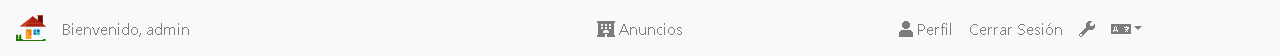
\includegraphics[width=1\textwidth]{Img/ManualUsuario/ADMIN_MENU.png}
\end{figure}

\subsection{Anuncios}
En la consulta de anuncios, el usuario administrador dispondr\'{a} de las siguientes opciones extra en el men\'{u} lateral, es decir: podr\'{a} modificar cualquier anuncio (aunque no lo haya publicado \'{e}l), eliminarlo y bloquearlo. El resto de opciones ser\'{a}n comunes al usuario registrado.

\begin{figure}[h!]
\centering
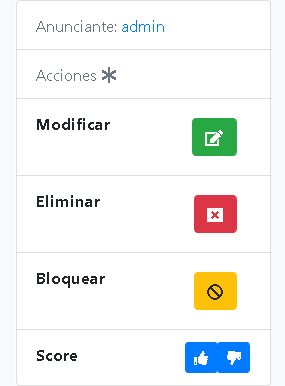
\includegraphics[width=.3\textwidth]{Img/ManualUsuario/ADS_ADMIN__PANEL.png}
\end{figure}

\subsection{Perfil de Usuario}
En la zona del perfil de usuario cabe mencionar que la visi\'{o}n ser\'{a} la misma que los usuarios registrados, con la salvedad de que, al consultar el perfil de otros usuarios (y que estos no sean administrador) se a\~{n}adir\'{a}n opciones de bloqueo y eliminaci\'{o}n.
\begin{figure}[h!]
\centering
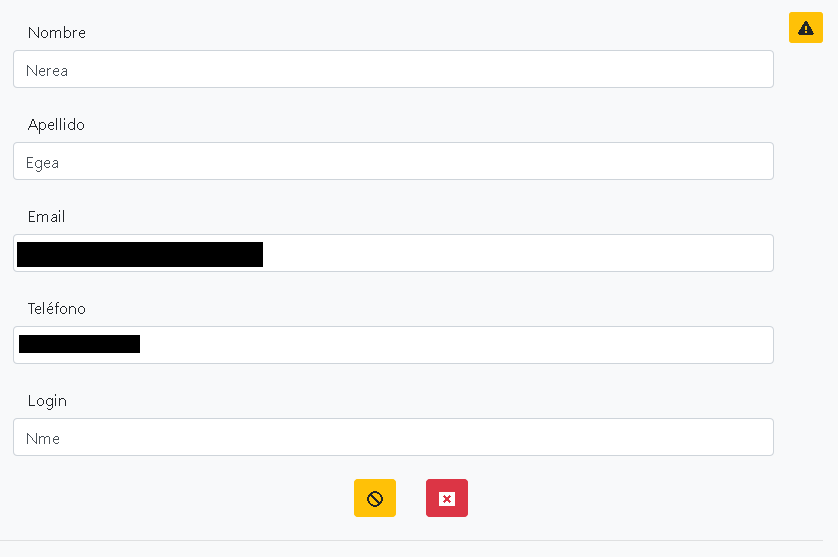
\includegraphics[width=.4\textwidth]{Img/ManualUsuario/ADMIN_SEARCH_USER.png}
\end{figure}


\subsection{Dashboard o panel de gesti\'{o}n}
La zona m\'{a}s importante y clave en el rol de administrador es la conocida como panel de gesti\'{o}n o Dashboard (cuadro de mando en ingl\'{e}s).  En esta parte de la aplicaci\'{o}n, el administrador dispondr\'{a} de 5 tipos de gesti\'{o}n: usuarios, anuncios, comentarios, tipos y denuncias.

\subsubsection{Gesti\'{o}n de Usuarios}
En la primera p\'{a}gina, por defecto, el usuario administrador podr\'{a} observar una gr\'{a}fica con las estad\'{i}sticas de los usuarios registrados por meses. A su derecha, un bot\'{o}n que permite crear usuarios desde el mismo cuadro de mando. Debajo de lo mencionado anteriormente, se tiene una tabla con los listados de los usuarios, mostrando id, nombre, apellido, email, rol y fecha de registro, adem\'{a}s de ofrecer la posibilidad de mostrar todos los datos al completo y gestionar editando, bloqueando o eliminando a los usuarios.

\begin{figure}[h!]
\centering
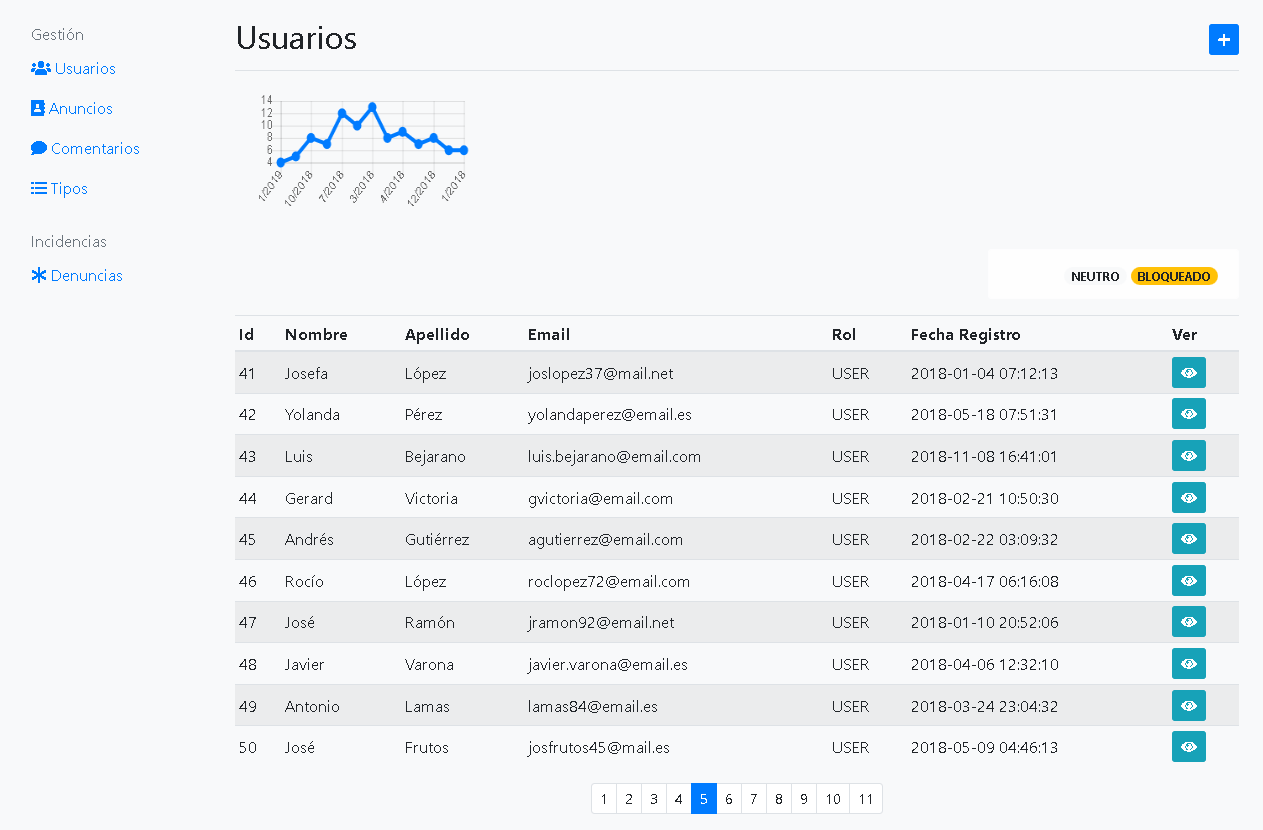
\includegraphics[width=.8\textwidth]{Img/ManualUsuario/ADMIN_DASHBOARD_USER.png}
\end{figure}

Al hacer click sobre el bot\'{o}n de creaci\'{o}n de usuarios se mostrar\'{a} un modal que solicite nombre, apellidos, email, tel\'{e}fono, login, contrase\~{n}a, su verificaci\'{o}n y el rol del usuario a crear. Esta \'{u}ltima petici\'{o}n se debe a la posibilidad de crear varios usuarios con el rol de administrador para que gestionen el sistema.


\begin{figure}[h!]
\centering
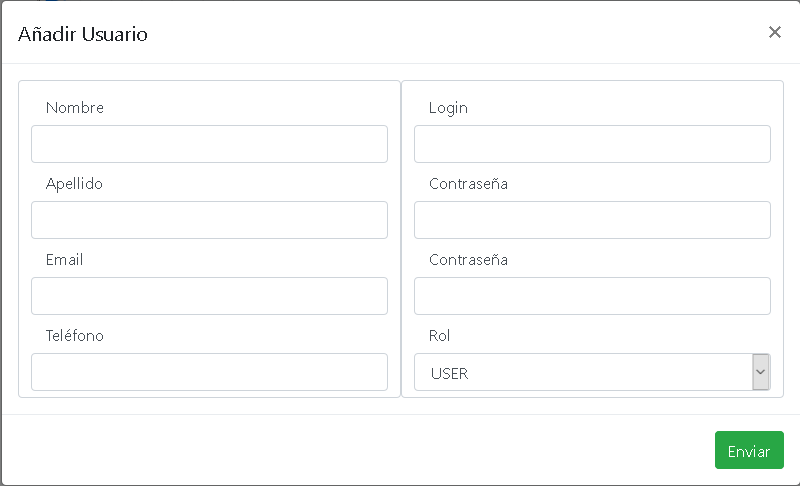
\includegraphics[width=.8\textwidth]{Img/ManualUsuario/ADMIN_CREATE_USER.png}
\end{figure}

Accediendo a la tabla de usuarios y accionando el bot\'{o}n para consultar los datos (Ver), se visualizar\'{a} una tabla con el id, uuid, nombre, apellidos, email, tel\'{e}fono, fecha de registro y rol, adem\'{a}s de tres posibles botones: bloquear, eliminar y editar. Bloquear ser\'{a} sustitu\'{i}do por desbloquear en caso de que el usuario en cuesti\'{o}n est\'{e} ya bloqueado. Tanto bloquear como eliminar no ser\'{a}n ofrecidos si el usuario consultado es administrador.



\begin{figure}[h!]
\centering
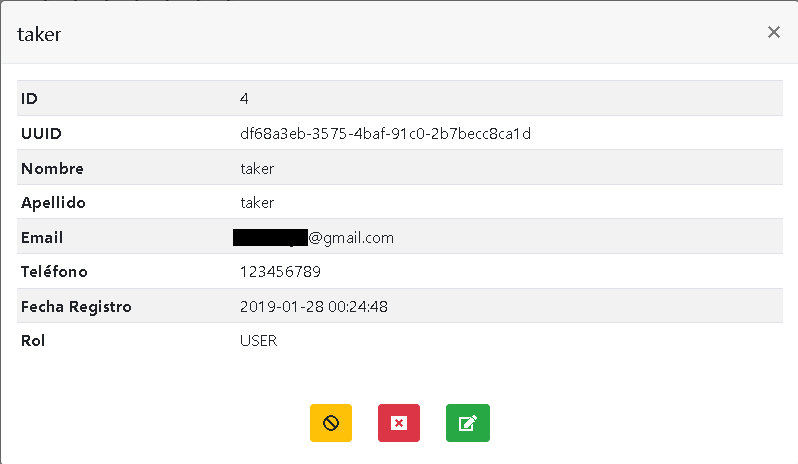
\includegraphics[width=.8\textwidth]{Img/ManualUsuario/ADMIN_READ_USER.png}
\end{figure}

Los modales que se mostrar\'{a}n para la confirmaci\'{o}n de bloqueo, desbloqueo y eliminaci\'{o}n ser\'{a} como el siguiente, variando en el mensaje de confirmaci\'{o}n.

\begin{figure}[h!]
\centering
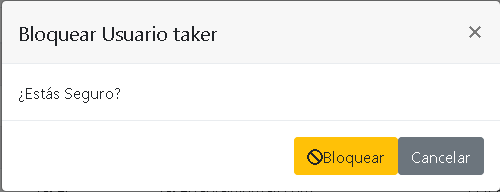
\includegraphics[width=.6\textwidth]{Img/ManualUsuario/ADMIN_BLOCK_USER.png}
\end{figure}

Si confirmara dicha acci\'{o}n de bloqueo,el usuario bloqueado tendr\'{i}a un tono amarillo en la tabla, adem\'{a}s de un mensaje avisando en su consulta.

\begin{figure}[h!]
\centering
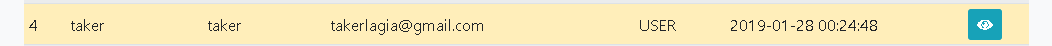
\includegraphics[width=1\textwidth]{Img/ManualUsuario/ADMIN_USER_BLOCKED.png}
\end{figure}

\begin{figure}[h!]
\centering
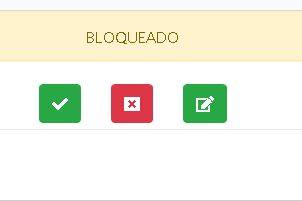
\includegraphics[width=.4\textwidth]{Img/ManualUsuario/ADMIN_BLOCKED_READ_USER.png}
\end{figure}

Si accionara el bot\'{o}n de editar usuario acceder\'{i}a a otro modal con el formulario que permitiera editar nombre, apellidos, tel\'{e}fono rol y contrase\~{n}a, verificando siempre esta \'{u}ltima en un segundo campo de contrase\~{n}a.


\begin{figure}[h!]
\centering
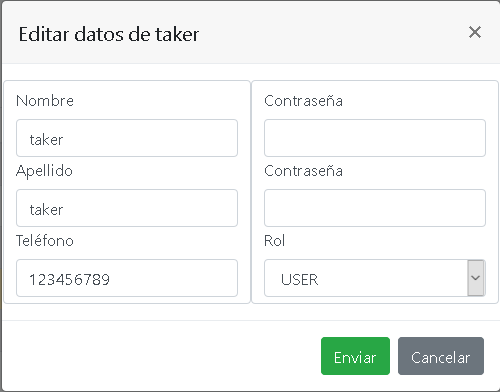
\includegraphics[width=.4\textwidth]{Img/ManualUsuario/ADMIN_EDIT_USER.png}
\end{figure}

\subsubsection{Gesti\'{o}n de Anuncios}
Para la gesti\'{o}n de anuncios, seleccionando en el men\'{u} lateral izquierdo en la opci\'{o}n 'Anuncios',  donde se ha decidido separar las consulta de los  listados, donde las opciones vistas en la secci\'{o}n anterior de anuncios para el administrador ser\'{a}n las ofrecidas para editarlos, modificarlos y bloquearlos o desbloquearlos.

\begin{figure}[h!]
\centering
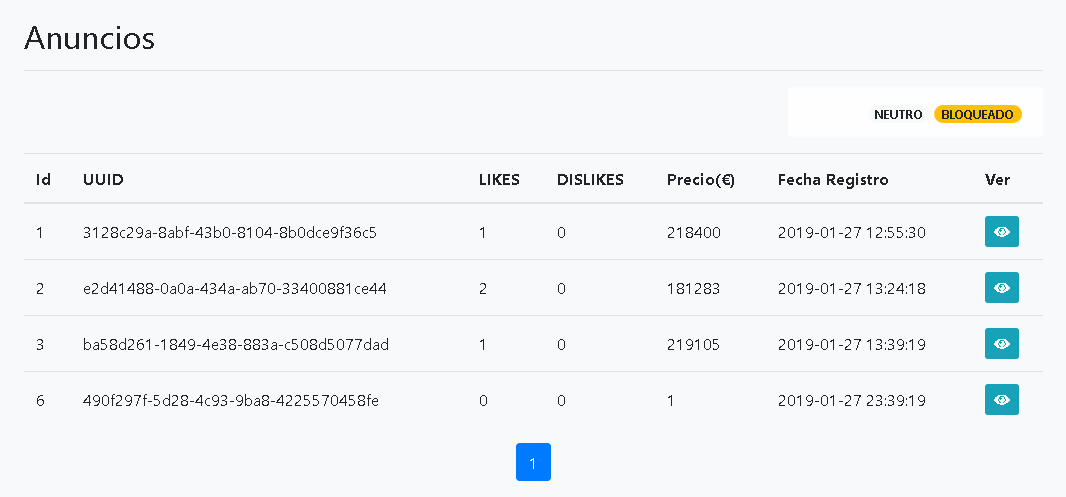
\includegraphics[width=.7\textwidth]{Img/ManualUsuario/ADMIN_ADS_DASHBOARD.png}
\end{figure}

En la tabla de anuncios se listan los id, uuid, n\'{u}mero de likes, dislikes, precio, fecha registro y la posibilidad de consultarlos, enviando a la p\'{a}gina com\'{u}n mencionada anteriormente.



\subsubsection{Gesti\'{o}n de Comentarios}
Haciendo click en la opci\'{o}n de 'Comentarios' el usuario administrador podr\'{a} acceder a la secci\'{o}n de administraci\'{o}n de los comentarios, observando una gr\'{a}fica con las mismas caracter\'{i}sticas que el mostrado en la zona de administraci\'{o}n de usuarios, en este caso mostrando la cantidad de mensajes agrupadas por mes y a\~{n}o. \\

De los comentarios se listan el id, el acceso al anuncio referenciado, el usuario que lo realiz\'{o}, el contenido, fecha de registro del mismo y la posibilidad de eliminarlo.

\begin{figure}[h!]
\centering
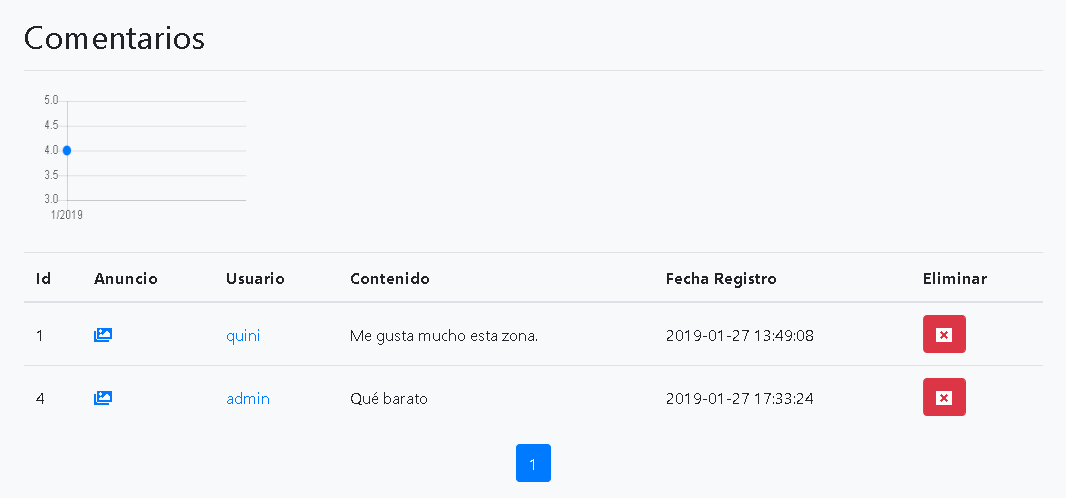
\includegraphics[width=.7\textwidth]{Img/ManualUsuario/ADMIN_COMMENT_DASH.png}
\end{figure}


\subsubsection{Gesti\'{o}n de Tipos}
Del mismo modo que en los anteriores puntos, el acceso a la gesti\'{o}n de tipos ofrecer\'{a} un listado, en este caso para cada tipo tratado en el sistema: tipos de vivienda y tipos de operaci\'{o}n. 

\begin{figure}[h!]
\centering
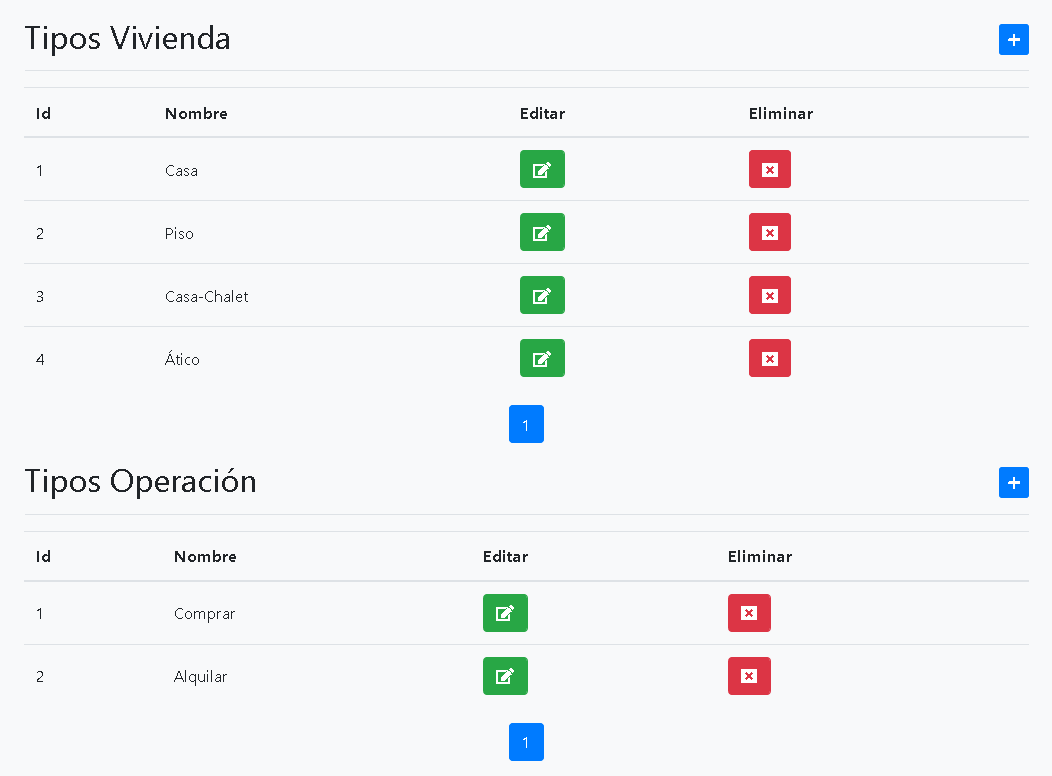
\includegraphics[width=.6\textwidth]{Img/ManualUsuario/ADMIN_TYPE.png}
\end{figure}

Para crear un tipo de vivienda, con hacer click en el bot\'{o}n con el s\'{i}mbolo $+$ en la zona superior derecha aparecer\'{a} un modal solicitando el nombre del nuevo tipo a crear.

\begin{figure}[h!]
\centering
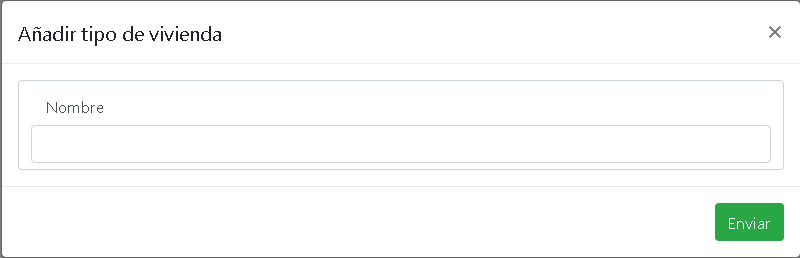
\includegraphics[width=.6\textwidth]{Img/ManualUsuario/ADMIN_CREATE_THOUSING_TYPE.png}
\end{figure}
 
En caso de seleccionar editar aparecer\'{a} un formulario similar:

\begin{figure}[h!]
\centering
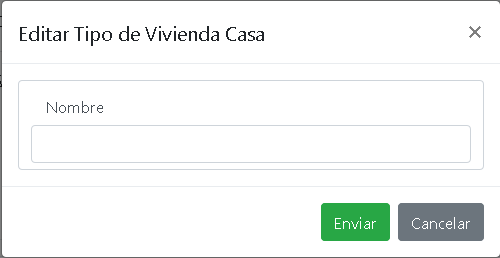
\includegraphics[width=.5\textwidth]{Img/ManualUsuario/ADMIN_EDIT_HOUSING_TYPE.png}
\end{figure}

Para eliminar se pedir\'{a} confirmaci\'{o}n con un modal similar al visto en la secci\'{o}n de usuarios.

En la tabla inferior se pueden observar las mismas prestaciones, cuyo uso ser\'{a} el mismo que el reci\'{e}n explicado.

\subsubsection{Gesti\'{o}n de Denuncias}
La gesti\'{o}n de denuncias agrupar\'{a} todos los tipos de denuncia por tablas, juntando en primer lugar las de usuario, seguidas de anuncios, comentarios y peticiones.

\begin{figure}[h!]
\centering
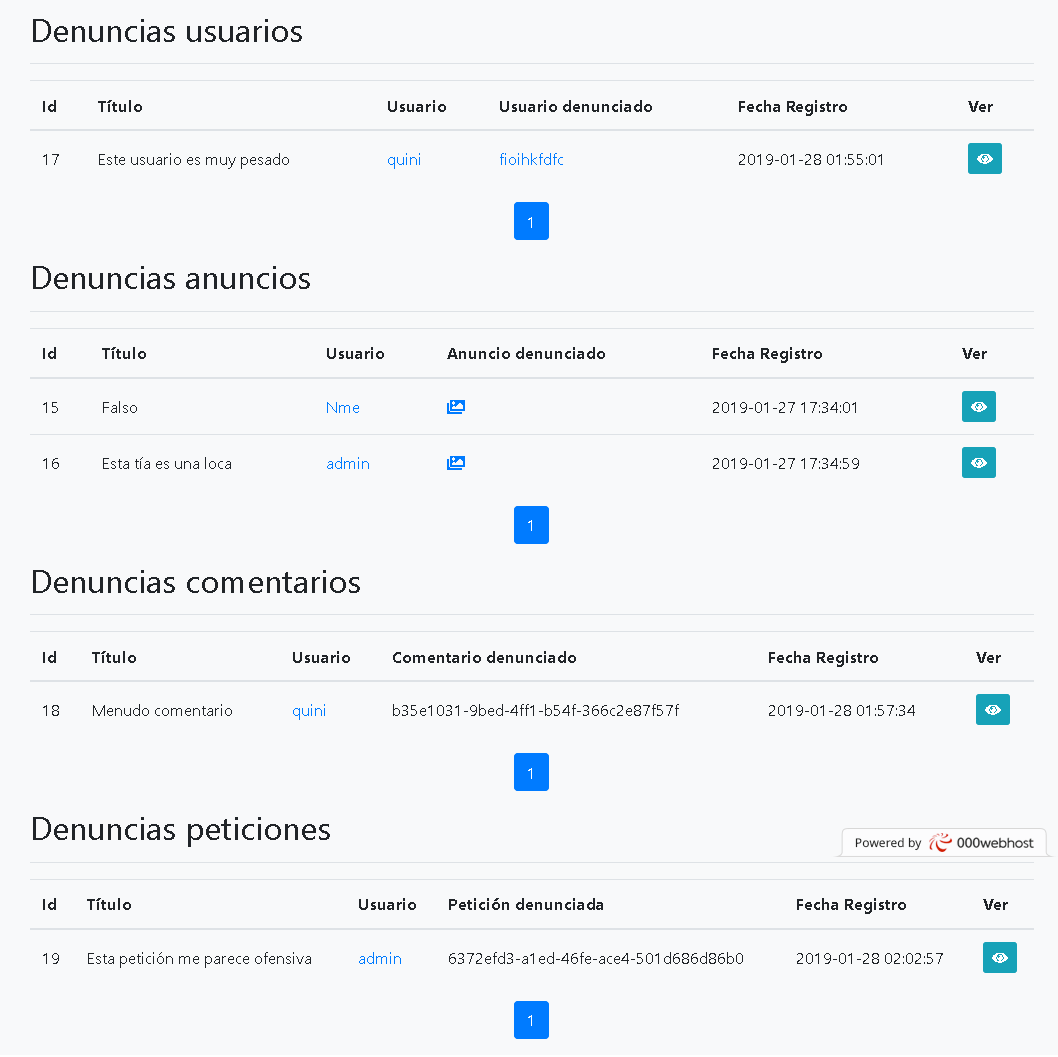
\includegraphics[width=.9\textwidth]{Img/ManualUsuario/DENUNCIAS_ADMIN.png}
\end{figure}


Las denuncias de usuarios presentan en el listado el id, t\'{i}tulo, referencia al usuario denunciante, referencia al usuario denunciado, fecha de registro y ampliaci\'{o}n o consulta de los detalles de la misma, en cuyo modal se encontrar\'{a} el id, uuid y los mismos datos mencionados en la lista. Debajo de estos la posibilidad de aceptar o rechazar la denuncia con dos botones. Aceptar una denuncia de usuario, se bloquear\'{a} del sistema al usuario denunciado y marcar\'{a} la denuncia como aceptada. Por otro lado, al rechazarla simplemente se descartar\'{a} y marcar\'{a} como rechazada.



\begin{figure}[h!]
\centering
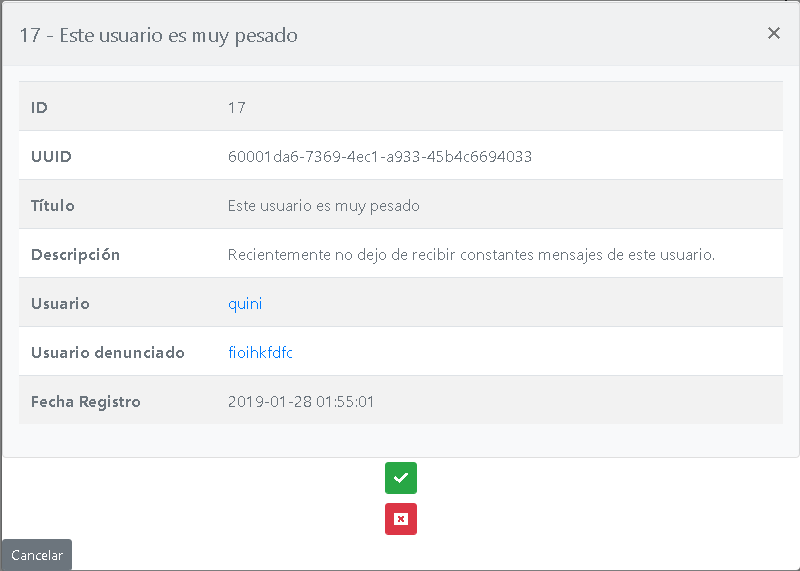
\includegraphics[width=.5\textwidth]{Img/ManualUsuario/ADMIN_SHOW_REPORT_USER.png}
\end{figure}


Las denuncias de anuncios presentan el id, t\'{i}tulo del mismo, referencia al usuario denunciante y al anuncio denunciado, fecha de registro y ampliaci\'{o}n de los datos, a\~{n}adiendo a los anteriores id, uuid, descripci\'{o}n y los botones anteriormente mencionados de aceptar y rechazar denuncia. Las denuncias de anuncios, al igual que las de usuarios, son bloqueantes.


\begin{figure}[h!]
\centering
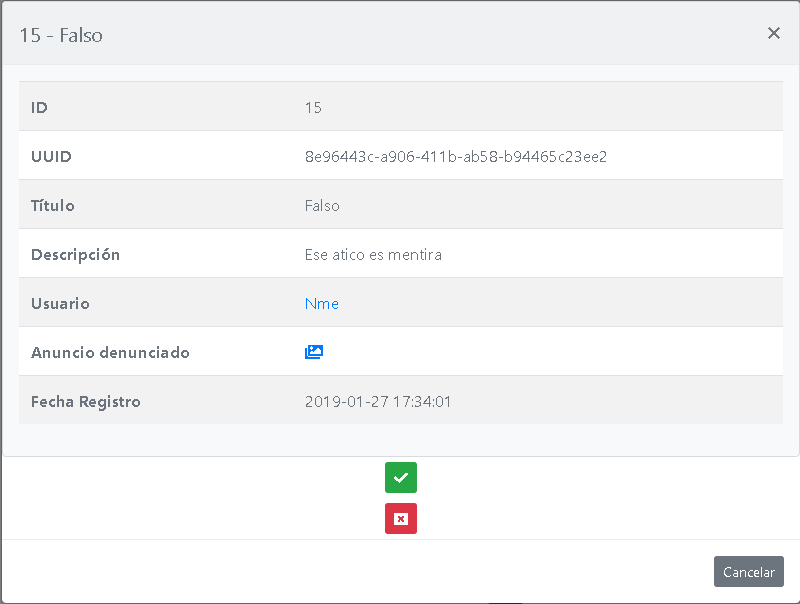
\includegraphics[width=.5\textwidth]{Img/ManualUsuario/ADMIN_SHOW_REPORT_AD.png}
\end{figure}

Los comentarios denunciados presentan las mismas caracter\'{i}sticas, es decir, un id, t\'{i}tulo, link al usuario denunciante, el uuid del comentario denunciado, fecha registro y acceso al detalle en 'ver'. En este caso el comentario denunciado no es referenciado directamente, pero se prevee que en futuras implementaciones se pueda hacer. El detalle de las denuncias de comentarios presenta id, uuid, t\'{i}tulo, descripci\'{o}n, link al usuario, contenido del comentario que fue denunciado y fecha registro, adem\'{a}s de los dos botones ya conocidos de aceptar y rechazar. Las denuncias de comentarios no bloquean al aceptar, como las de usuarios y anuncios. En su lugar, se borra del sistema.

\begin{figure}[h!]
\centering
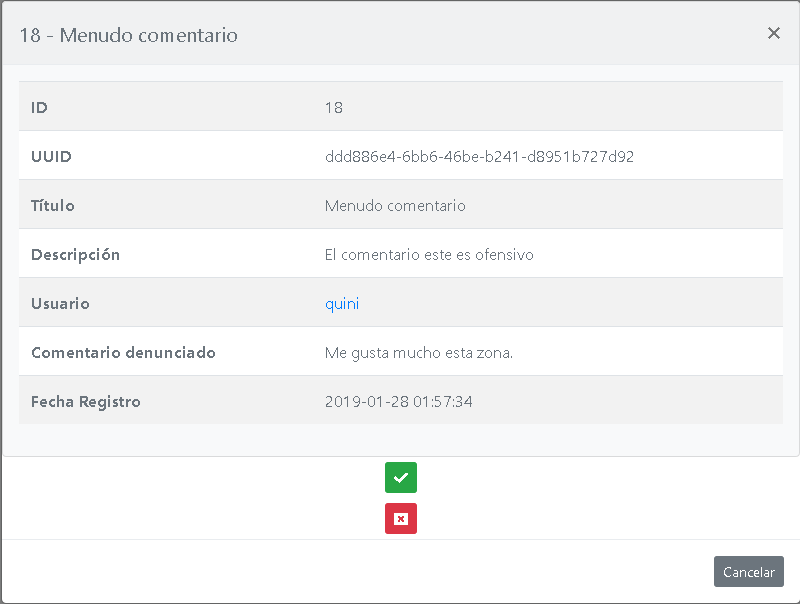
\includegraphics[width=.5\textwidth]{Img/ManualUsuario/ADMIN_SHOW_REPORT_COMMENT.png}
\end{figure}

En \'{u}ltimo, lugar, pero no menos importante por ello, se tiene el listado de denuncias de peticiones, mostrando el id, t\'{i}tulo y referencia al usuario denunciante nuevamente, uuid de la petici\'{o}n denunciada, fecha registro y ampliaci\'{o}n en 'ver'. Al igual que las anteriores, el contenido de la tarjeta con los detalles contendr\'{a} id, uuid, t\'{i}tulo, descripci\'{o}n, link al perfil del usuario denunciante,  contenido de la petici\'{o}n denunciada (es decir, el mensaje que escribi\'{o} el usuario cuya petici\'{o}n fue denunciada), fecha registro y los botones de aceptar o rechazar.Al igual que los comentarios, se borrar\'{a}n las peticiones cuyas denuncias asociadas sean aceptadas.


\begin{figure}[h!]
\centering
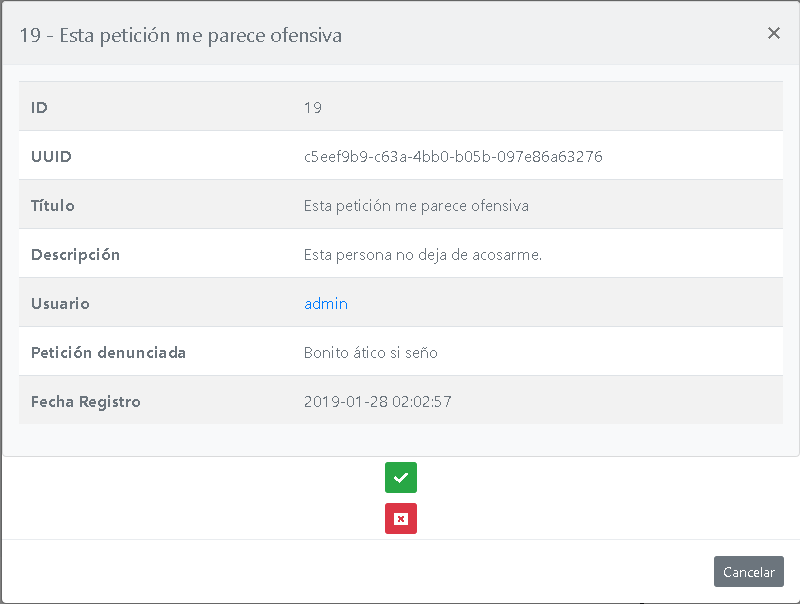
\includegraphics[width=.5\textwidth]{Img/ManualUsuario/ADMIN_SHOW_REPORT_REQUEST.png}
\end{figure}